\documentclass[a4paper,11pt]{amsbook}
%\usepackage[utf8]{inputenc}


\usepackage{amsmath, amscd, amssymb, amsthm, latexsym}
\usepackage[usenames,dvipsnames,table]{xcolor}
\usepackage{graphicx}
\usepackage{cite}
\usepackage{fontspec}
\setmainfont[SmallCapsFont = Fontin SmallCaps]{Fontin}
\usepackage{tikz}
\usetikzlibrary{calc}
\usepackage{hyperref}
\usepackage{clrscode3e}
\usepackage{import}
%\usepackage{fullpage}
% \usepackage{clrscode3e}	--algun paquete de algoritmos
\newtheorem{defn}{Definition}
\newtheorem{prop}{Proposition}
\newtheorem{thm}{Theorem}
\newtheorem{lem}{Lemma}
\newtheorem{cor}{Corollary}
\newtheorem{obs}{Observation}
\newtheorem{eg}{Example}

%For \autoref to add the word before number
\newcommand*{\defnautorefname}{Definition}
\newcommand*{\propautorefname}{Proposition}
\newcommand*{\thmautorefname}{Theorem}
\newcommand*{\lemautorefname}{Lemma}
\newcommand*{\corautorefname}{Corollary}
\newcommand*{\obsautorefname}{Observation}
\newcommand*{\egautorefname}{Example}
\def\sectionautorefname{Section}
\def\chapterautorefname{Chapter}

\tikzset{
  v/.style={draw, circle, inner sep=0pt, font=\small, align=center, minimum size=0.75cm},
  e/.style={->, dashed}
}
\newcommand{\dottedarrow}[2]{\draw[e] ($(#1)!0.5cm!(#2)$) -> ($(#1)!1cm!(#2)$)}
\newcommand{\dottedarrows}[4]{
  \foreach \i in #1 {
    \foreach \j in #2 {
      \ifnum\pdfstrcmp{\i}{#3}=0
        \ifnum\pdfstrcmp{\j}{#4}=0
        \else
          \dottedarrow{\i}{\j};
        \fi
      \else
        \dottedarrow{\i}{\j};
      \fi
    }
  }
}

\newlength{\problemoffset}
\setlength{\problemoffset}{0.5in}
\newcommand{\decision}[3]{%     \decision{NAME}{INSTANCE}{QUESTION}
\begin{list}{}{
\setlength{\leftmargin}{\problemoffset}
\setlength{\rightmargin}{\problemoffset}
\setlength{\parsep}{0pt}
\setlength{\itemsep}{2pt}
\setlength{\topsep}{\itemsep}
\setlength{\partopsep}{\itemsep}
}
\item
{\textsc{#1}}
\item
{INSTANCE: #2}
\item
{QUESTION: #3}
\end{list}
}

\definecolor{light-gray}{gray}{0.75}

\newcommand{\bigoh}{\ensuremath{\mathcal{O} }}
\newcommand{\N}{\mathbb{N}}
\newcommand{\Nz}{\mathbb{N}_0}
\newcommand{\Z}{\mathbb{Z}}
\newcommand{\Q}{\mathbb{Q}}
\newcommand{\R}{\mathbb{R}}
%\newcommand{\G}{\mathcal{G}}
\newcommand{\Parts}{\mathcal{P}}
\newcommand{\dist}{{\rm dist}}
\newcommand{\adj}{{\rm Adj}}
\newcommand{\symdiff}{\bigtriangleup}
\newcommand{\npc}{\ensuremath{\mathcal{NP}{\text{-complete}}} }
\newcommand{\npces}{\ensuremath{\mathcal{NP}{\text{-completo}}} }
\newcommand{\nph}{\ensuremath{\mathcal{NP}{\text{-hard}}} }
\newcommand{\np}{\ensuremath{\mathcal{NP}} }
\newcommand{\p}{\ensuremath{\mathcal{P}} }
\newcommand{\gic}{\ensuremath{\mathcal{GI}{\text{-complete}}} }
\newcommand{\gih}{\ensuremath{\mathcal{GI}{\text{-hard}}} }
\newcommand{\gi}{\ensuremath{\mathcal{GI}} }
\newcommand{\mcesp}{{\textsc{MCESP} }}
\newcommand{\mincesp}{{\textsc{MinCESP} }}
\newcommand{\maxcut}{{\textsc{Max-Cut} }}
\newcommand{\yes}{{\textsc{Yes}} }
\newcommand{\no}{{\textsc{No}} }
\DeclareMathOperator{\tr}{tr}
\newcommand{\todo}[1]{\textcolor{red}{TODO : #1}}
\newcommand{\note}[1]{\textcolor{blue}{NOTA : #1}}
\newcommand{\HRule}{\rule{\linewidth}{0.5mm}}
\renewcommand\qedsymbol{\ensuremath{\blacksquare}}
\renewcommand*{\subsectionautorefname}{Subsection}
\newcommand\restr[2]{{% we make the whole thing an ordinary symbol
  \left.\kern-\nulldelimiterspace % automatically resize the bar with \right
  #1 % the function
  \vphantom{\big|} % pretend it's a little taller at normal size
  \right|_{#2} % this is the delimiter
  }}


\hypersetup{
linkcolor = blue,
colorlinks = true,
citecolor = magenta
}

\DeclareRobustCommand{\gobblefive}[5]{}
\newcommand*{\SkipTocEntry}{\addtocontents{toc}{\gobblefive}}


\begin{document}
\numberwithin{section}{chapter}
\setcounter{section}{1}
%\numberwithin{subsection}{section}
\numberwithin{prop}{section}
%\numberwithin{prop}{subsection}
\numberwithin{lem}{section}
%\numberwithin{lem}{subsection}
\numberwithin{thm}{section}
%\numberwithin{thm}{subsection}
\numberwithin{cor}{section}
%\numberwithin{cor}{subsection}
\numberwithin{defn}{section}
%\numberwithin{defn}{subsection}
\numberwithin{equation}{section} %sets equation numbers <chapter>.<section>.<index>
%\numberwithin{equation}{subsection} %sets equation numbers <chapter>.<section>.<subsection>.<index>
%\numberwithin{equation}{subsubsection} %sets equation numbers <chapter>.<section>.<subsection>.<subsubsection>.<index>
\numberwithin{obs}{section} %sets equation numbers <chapter>.<section>.<index>
%\numberwithin{obs}{subsection} %sets equation numbers <chapter>.<section>.<subsection>.<index>
\numberwithin{figure}{section} %sets equation numbers <chapter>.<section>.<index>
%\numberwithin{figure}{subsection} %sets equation numbers <chapter>.<section>.<subsection>.<index>
%\maketitle

\begin{titlepage}

\begin{center}


% Upper part of the page
\begin{flushleft}
\raisebox{-.5\height}{
\includegraphics[width=13em]{./graphics/logofcen}}%
\hfill
\raisebox{-.5\height}{
\includegraphics[width=15em]{./graphics/dc_logo}}\\[2.0cm]
\end{flushleft}

{\large \sc Universidad de Buenos Aires

Facultad de Ciencias Exactas y Naturales

Departamento de Computaci\'on} \\[2cm]

% Title
%\HRule \\[0.4cm]
{ \LARGE \bfseries Complexity and polyhedral studies of a course scheduling and professor assignment problem}\\[2.6cm]
%\HRule \\[1.2cm]
{\large Tesis presentada para optar al t\'{\i}tulo de\\
Licenciado en Ciencias de la Computaci\'on}
\vfill
% Author and supervisor
{\large \emph{Autor:} Federico \textsc{Lebrón}\\[0.5cm]
\emph{Director:} 
Dr.~Javier \textsc{Marenco} \\[0.5cm]
\emph{Jurados:} 
Dr.~Min Chih \textsc{Lin} y 
Dra.~Isabel \textsc{Méndez-Díaz}
}
\vfill

{\large \today}

\end{center}
\end{titlepage}

\setcounter{tocdepth}{3} %temporal

\pagenumbering{roman}
%\SkipTocEntry \chapter*{Abstract}
%Los problemas de asignación de horarios han sido ampliamente estudiados en la literatura de investigación operativa. Esta importante parte del planeamiento de cursos es conocida por ser particularmente difícil, ambas en la teoría y en la práctica, en varios casos importantes. Es por esta razón que es estudiado por la comunidad de la optimización combinatoria. En particular, es estudiado usando modelos de programación lineal entera.

En este trabajo consideramos una versión de este problema y la estudiamos tanto desde el punto de vista teórico como el práctico. Llamamos a esta variación el Problema de Asignación de Cursos y Profesores (CSPAP por su sigla en inglés). Las restricciones que consideramos son las de disponibilidad de los profesores, roles que pueden ocupar, variabilidad de fechas de inicio de los cursos, y variabilidad de patrones semanales de los cursos. Estudiamos el cambio de fase en la complejidad computacional cuando algunas de estas restricciones son aplicadas o levantadas, y vemos cómo el problema pasa de pertenecer a la clase $\p$ a la clase $\npces$.

Para el problema general, consideramos un enfoque poliedral, que produce resultados eficientes para problemas de tamaños prácticos. Para instancias de tamaños más grandes, el rendimiento decae. Por este motivo desarrollamos familias de desigualdades válidas, aumentando la eficiencia de los algoritmos de tipo branch-and-bound de programación lineal entera. Al utilizar estas desigualdades, problemas de tamaño práctico son resueltos en cuestión de segundos.

\SkipTocEntry \chapter*{Abstract}
The course scheduling and professor assignment problem (CSPAP) consists of constructing a timetable and assigning professors to classes, subject to some restrictions. This important part of course planning is known to be exceedingly hard, both in theory and in practice, in several important cases. For this reason it's been studied by the combinatorial optimization community. In particular, it's been studied using integer linear programming models.

In this work we consider one version of the problem and proceed to study it, both from a theoretical and practical standpoint. The restrictions we consider are ones of availability of faculty, course start date, and weekly course pattern. We study the complexity phase change that occurs when some restrictions are lifted or applied, and see how the problem shifts from \p to \npc.

For the general problem, we consider a polyhedral approach, and find cuts to increase the efficiency of a branch-and-cut integer linear programming solver.

%\SkipTocEntry \chapter*{Acknowledgments}
%blahblah


\tableofcontents
\newpage
\pagenumbering{arabic}
\subimport{chapters/1/}{main}
\documentclass{article}
\usepackage{tikz}
\usetikzlibrary{calc}
\usepackage{amsmath}
\usepackage{amssymb}
\usepackage[margin=1in]{geometry}

\begin{document}
\section{Complexity of reduced cases}
\subsection{Single course, single start date, single weekly pattern}

This case can be solved in polynomial time. Indeed, it is a simple case of a maximum-cost maximum-flow problem. Specifically, if we let \begin{itemize}
\item $p$ be the number of professors,
\item $d$ be the number of days,
\item $m$ be the number of roles, and
\item $n'_{i, k}$ be the number of professors of role $k$ that are needed on whichever class falls on the $i$th day
\end{itemize}

we can create the following flow network, where capacities are in blue, and costs are in red:

\vspace{10pt}

\begin{center}
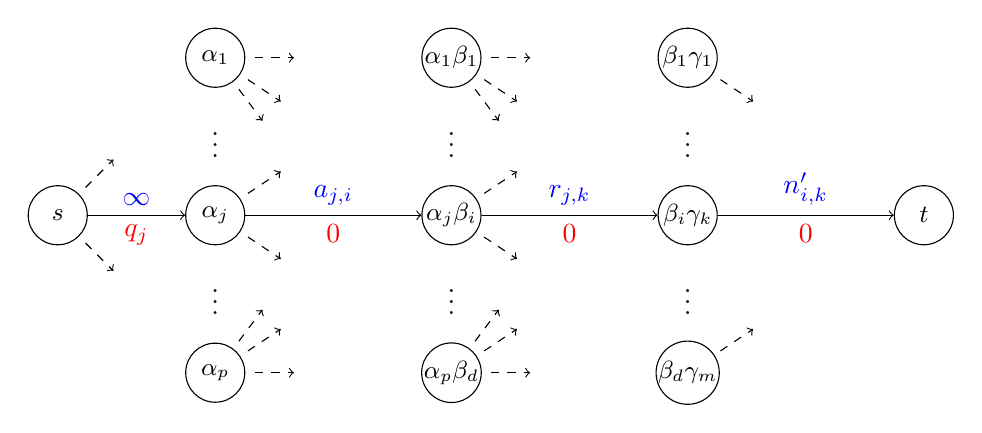
\begin{tikzpicture}

\tikzstyle{v}=[draw, circle, inner sep=0pt, font=\small, align=center, minimum size=0.75cm];
\tikzstyle{e}=[->, dashed];
\node[v] (s) at (1, 1) {$s$};
\node[v] (p_j) at (3, 1) {$\alpha_j$};
\node (d1) at (3, 2) {$\vdots$};
\node (d2) at (3, 0) {$\vdots$};
\node[v] (d3) at (3, 3) {$\alpha_1$};
\node[v] (d4) at (3, -1) {$\alpha_p$};

\node[v] (p_jd_i) at (6, 1) {$\alpha_j \beta_i$};
\node (d5) at (6, 0) {$\vdots$};
\node (d6) at (6, 2) {$\vdots$};
\node[v] (d7) at (6, 3) {$\alpha_1 \beta_1$};
\node[v] (d8) at (6, -1) {$\alpha_p \beta_d$};

\node[v] (d_ir_k) at (9, 1) {$\beta_i \gamma_k$};
\node (d9) at (9, 0) {$\vdots$};
\node (d10) at (9, 2) {$\vdots$};
\node[v] (d11) at (9, 3) {$\beta_1 \gamma_1$};
\node[v] (d12) at (9, -1) {$\beta_d \gamma_m$};

\node[v] (t) at (12, 1) {$t$};

\draw[->] (s) to node[above,blue] {$\infty$} node[below,red] {$q_j$} (p_j);

\dottedarrows{{s}}{{d3, d4}};

\draw[->] (p_j) to node[above,blue] {$a_{j, i}$} node[below,red] {$0$} (p_jd_i);

\dottedarrows{{d3, d4, p_j}}{{d7, p_jd_i, d8}}{p_j}{p_jd_i};

\draw[->] (p_jd_i) to node[above,blue] {$r_{j, k}$} node[below,red] {$0$} (d_ir_k);

\dottedarrows{{d7, d8, p_jd_i}}{{d11, d12, d_ir_k}}{p_jd_i}{d_ir_k};

\draw[->] (d_ir_k) to node[above,blue] {$n'_{i, k}$} node[below,red] {$0$} (t);

\dottedarrows{{d11, d12}}{{t}};

\end{tikzpicture}
\end{center}

Formally, the network is $G = (V, E)$, with

\begin{align*}
V = &\{s\} \cup \{t\}\\
&\cup \{\alpha_j \mid 1 \le j \le p\}\\
&\cup \{\alpha_j \beta_i \mid 1 \le j \le p, 1 \le i \le d\}\\
&\cup \{\beta_i \gamma_k \mid 1 \le i \le d, 1 \le j \le m\}\\
E = &\{(s, \alpha_j)\ \forall\ j\}\\
    &\cup \{(\alpha_j, \alpha_j \beta_i)\ \forall\ i, j \}\\
    &\cup \{(\alpha_j \beta_i, \beta_i \gamma_k)\ \forall\ j, i, k\}\\
    &\cup \{(\beta_i \gamma_k, t)\ \forall\ i, k \}
\end{align*}

capacity function $c:E \to \mathbb{R} \cup \{\infty\}$, such that
\begin{align*}
c(s, \alpha_j) &= \infty\ \forall\ j\\
c(\alpha_j, \alpha_j \beta_i) &= a_{j, i}\ \forall\ i, j\\
c(\alpha_j \beta_i, \beta_i \gamma_k) &= r_{j, k}\ \forall\ i, j, k\\
c(\beta_i \gamma_k, t) &= n'_{i, k}\ \forall\ i, k
\end{align*}

and cost function $w:E \to \mathbb{R}$, such that

$$
w(e) =
\begin{cases}
q_j &\text{ if } e = (s, a_j) \text{ for some }j\\
0 & \text{otherwise}
\end{cases}
$$

We can think of the flow in this network as ``time'' dedicated by a professor at a given day, on a given role. A unit of flow goes from a professor to a given day (only if that professor is available that day), and to a given role (only if the professor could fit that role), and into fulfilling that day's quota for that role.

A professor cannot teach on an unavailable day, since flow can only go from the $j$th professor to the $i$th day if $a_{i, j} = 1$, and only one unit may go through in that case. This last fact ensures a professor cannot work twice in a single day, even under different roles.

He also cannot work in a role that is unavailable to him, since in order for flow to go from $\alpha_j \beta_i$ to $\beta_i \gamma_k$, meaning ``the $j$th professor teaches on the $i$th day'' to ``the $i$th day has one $k$th role position covered'', unless $r_{j, k} = 1$, so one cannot consider an instance of that role covered for that day unless the professor from which that unit of flow came indeed can work in that role.

Lastly, the number of instances of the $k$th role that a given $\beta_i \gamma_k$ needs for the $i$th day can not be greater than $n'_{i, k}$.

A flow $f$ in $G$ will be a valid assignment of professors exactly when $f(s, t) \ge \sum_{i, k} n'_{i, k}$. The constraints going into $t$ guarantee this implies $f(\beta_i \gamma_k, t) = r_{i, k}\ \forall i, k$, which means each day's requirements of each role are met.

In such a solution, if a unit of flow goes from $s$, to $\alpha_j$, through $\alpha_j \beta_i$, then through $\beta_i \gamma_k$, and finally to $t$, we consider that the $j$th professor teaches on the $i$th day with the $k$th role. The quality of this assignment is thus $q_j$.

Furthermore, to obtain an optimal solution, that is, a maximum sum of the qualities of the assignments, we need to maximize the cost of this flow, because this will mean the maximum value of the units going into (hence out of) the $\alpha_j$, which is the quality of the assignments we are making.

Since maximum-cost maximum-flow on $G$ is in $O(poly(|V|, |E|))$, and we can see our $|V|$ and $|E|$ are polynomials in $p, d, m$, we coclude this reduction can be solved in time $O(poly(p, d, m))$, and thus is in \textsc{P}.

\end{document}


\bibliography{references}{}
\bibliographystyle{plain}


\end{document}
